%%%%%%%%%%%%%%%%%%%%%%%%%%%%%%%%%%%%%%%%%%%%%%%%%%%%
%    Harvard Data Science Review Latex Template    %
%%%%%%%%%%%%%%%%%%%%%%%%%%%%%%%%%%%%%%%%%%%%%%%%%%%%

\PassOptionsToPackage{colorinlistoftodos}{todonotes}
\documentclass[]{hdsr}

%Graphics should all go in the figs/ directory
\graphicspath{{figs/}{../figs/}}

\usepackage{xcolor}
\usepackage{hyperref}
\usepackage{xurl}
\usepackage{cleveref}

\newcommand{\TODO}[1]{{\color{red} {\bf TODO:~}#1}}
\newcommand{\verify}[1]{{\textcolor{red}{#1}}}
\newcommand{\shorten}[1]{{\color{gray}{#1}}}
\newcommand{\lx}[1]{{\color{violet}{#1}}}

%\setlength{\marginparwidth}{2.5cm}
% Define a custom font size (e.g., 6pt font with 7pt line spacing)
%\newcommand{\customnotesize}{\fontsize{6pt}{7pt}\selectfont}
\newcommand{\lxnote}[1]{\todo[linecolor=violet,backgroundcolor=violet!25,bordercolor=violet,size=footnotesize]{#1}}


\begin{document}

% Larger bottom margin for the first page
\newgeometry{bottom=1.5in}

% Editorial staff will replace the following values:
% 1. Volume number
% 2. Issue number
% 3. Article DOI
% e.g. for Volume 2, Issue 3, DOI 12.345:
% \volumeheader{2}{3}{12.345}
\volumeheader{0}{0}{00.000}



\begin{center}

  \title{Article Proposal: Portraying the Many Facets of Impact with Influence Flowers}
  \maketitle

  % Start page numbering on second page. Must appear *after* \maketitle
  \thispagestyle{empty}

  \vspace*{.2in}

  % Authors and Affiliations
  \begin{tabular}{cc}
    Minjeong Shin\upstairs{1}, Lexing Xie\upstairs{1}
   \\[0.25ex]
   {\small \upstairs{1} School of Computing, The Australian National University, Canberra, Australia} \\
  \end{tabular}

  % Replace with corresponding author email address
  % \emails{
  %   \upstairs{*}correspondingauthor@example.edu
  %   }
  % \vspace*{0.4in}

\begin{figure}[H]
    \centering
    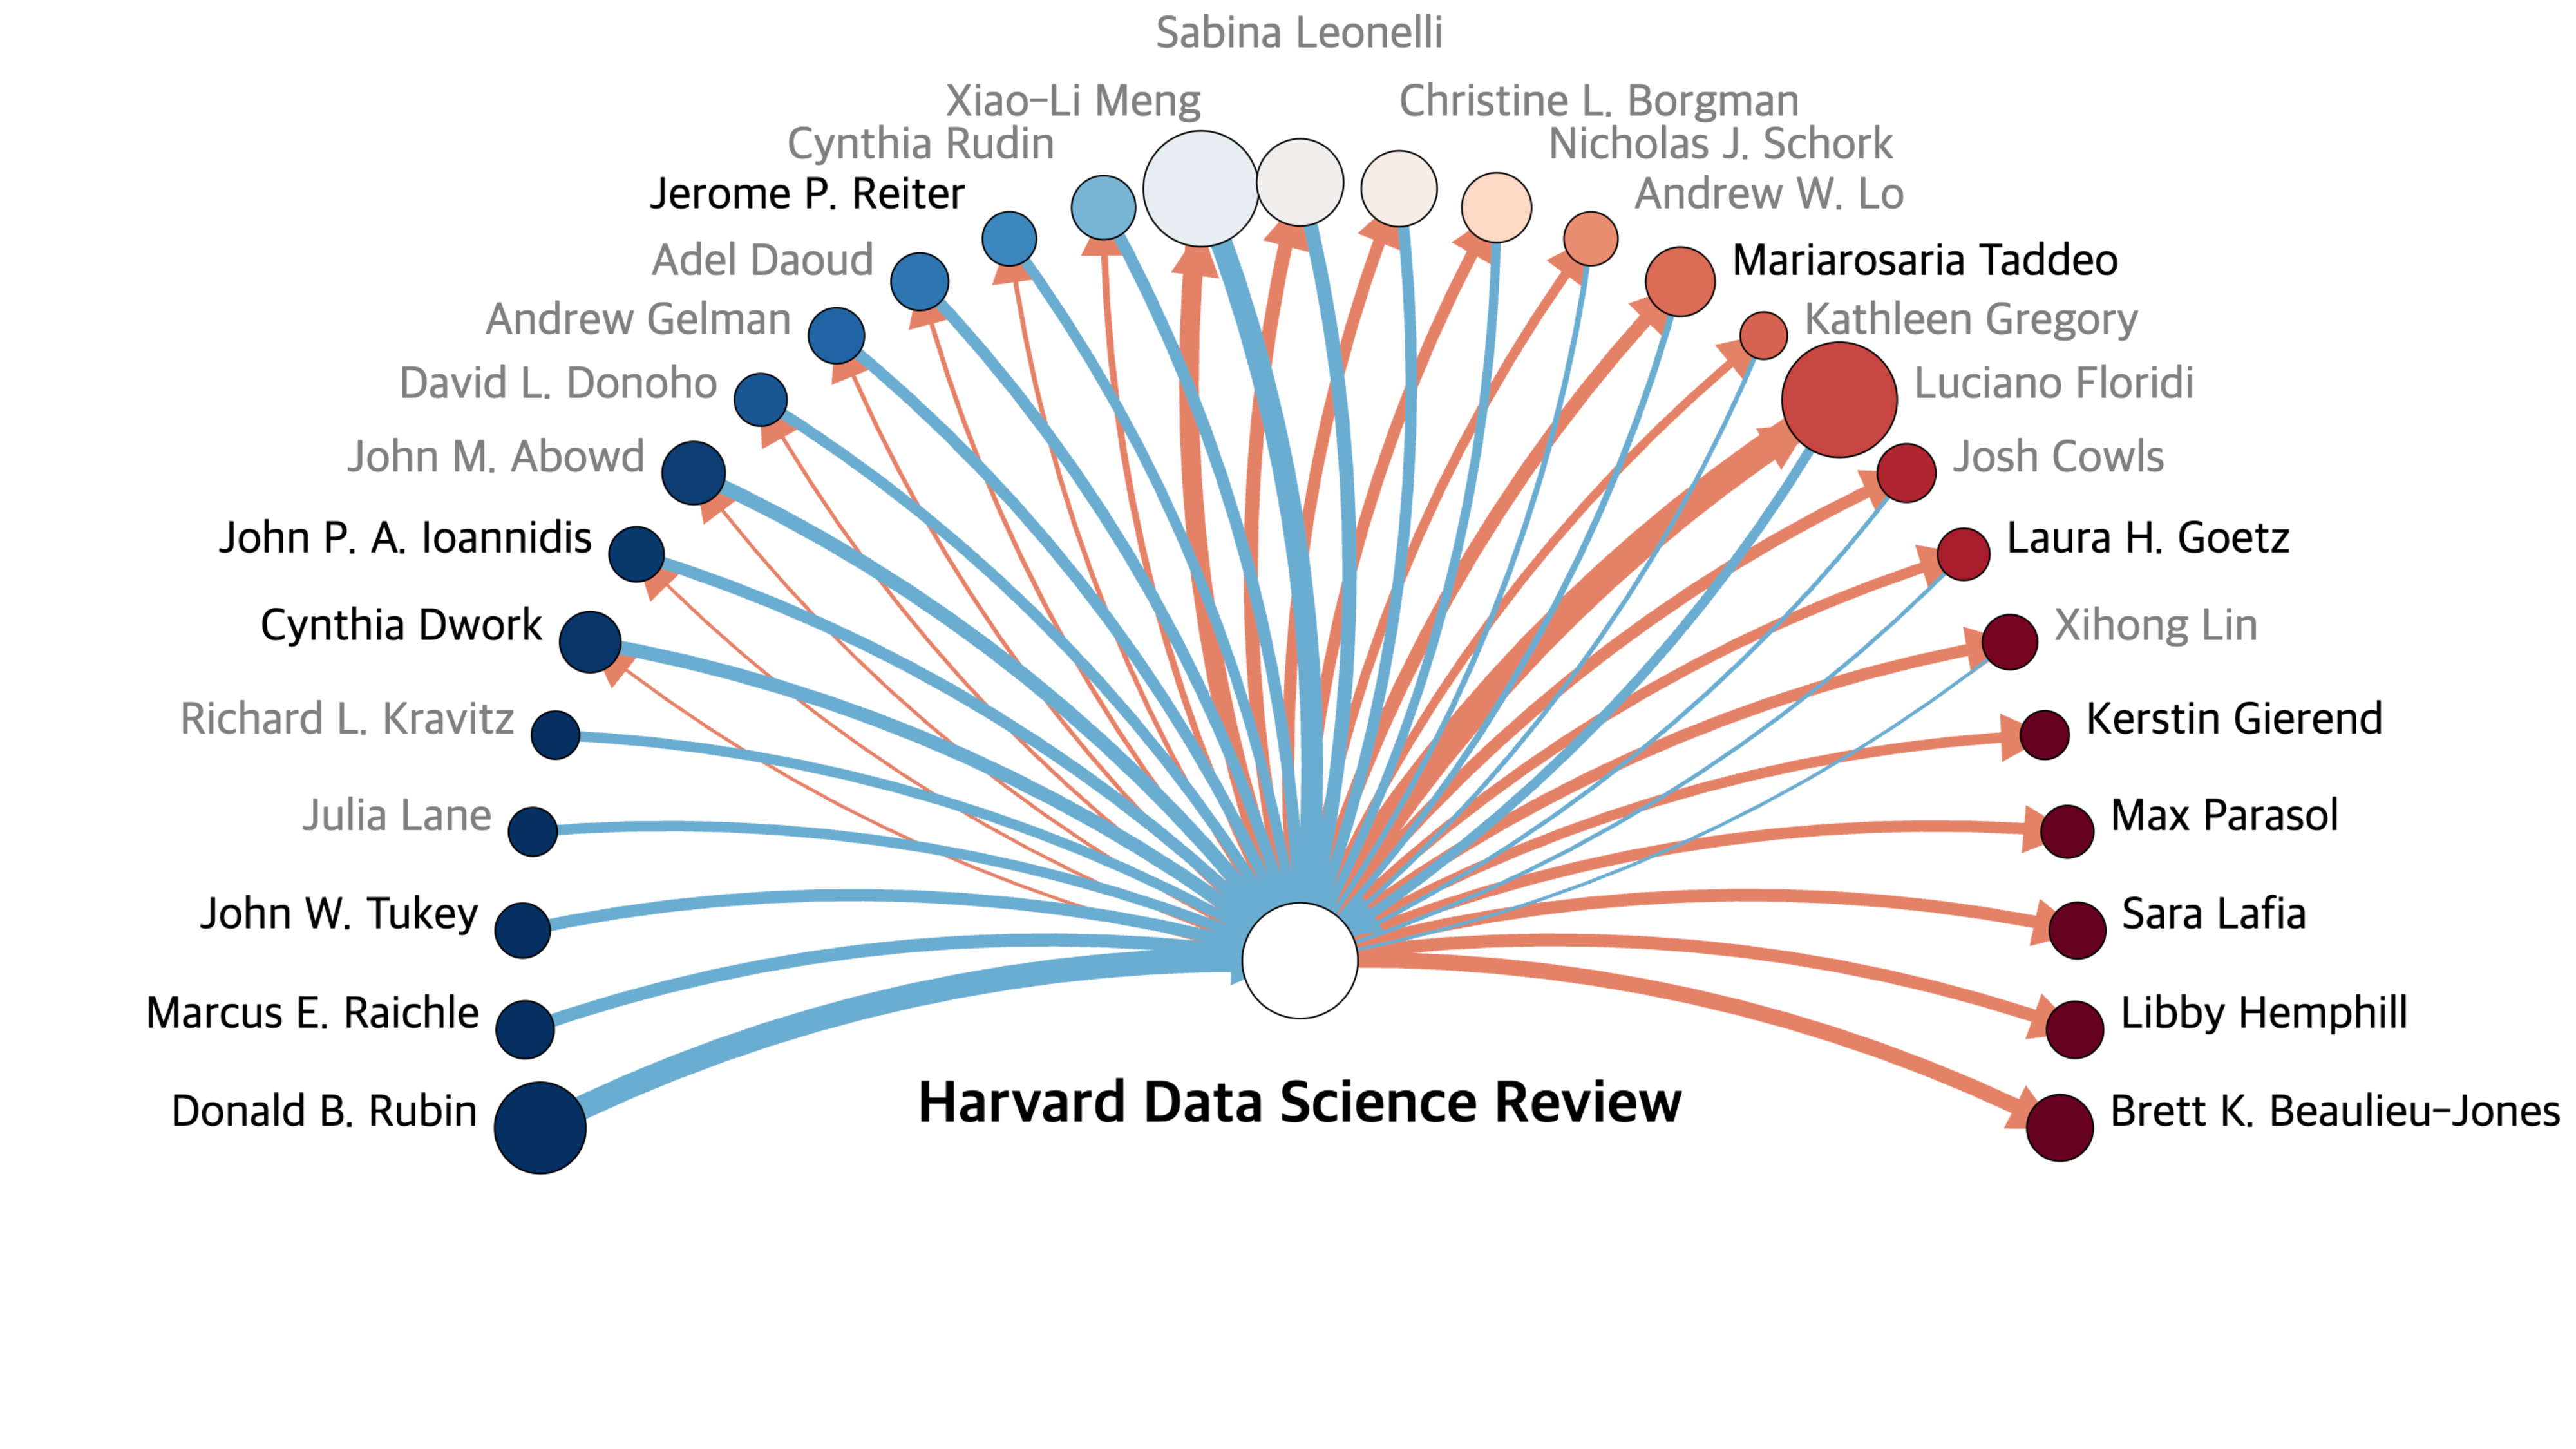
\includegraphics[width=0.9\textwidth]{hdsr_flower.pdf} \\
    \caption{\textbf{An influence flower visualization for HDSR (2019 to 2024)}, an {\href{https://influencemap.cmlab.dev/submit/?id=BAAAAAEAsCg5}{interactive version}} is available online. \textcolor{blue}{Blue arcs} denote incoming influence from the authors to papers in HDSR, with their thickness proportional to the number of references made. \textcolor{red}{Red arcs} denote outgoing influence from to papers in HDSR to the authors, with their thickness proportional to the number of citations received. Node color reflects the relative proportion of incoming vs outgoing influences. Greyed author names have published in HDSR.}
    \label{fig:hdsr_flower}
\end{figure}

% \begin{abstract}
% The abstract should be no more than 250 words.
% \end{abstract}


\vspace*{0.15in}
\hspace{10pt}
  \small
  \textbf{\textit{Keywords: }} {science of science, information visualization}\\
  \textbf{\textit{Possible HDSR Columns: }} {Meta Data Science, Diving into Data, Bits and Bytes}
% \copyrightnotice
\end{center}
\vspace*{0.15in}

% \section*{Media Summary}
% The Media Summary should be written in plain language to highlight the key messages of
% the article, in ways that can be understood by the general public and cited by the media
% directly and accurately.  It therefore should avoid technical terms or language designed for
% academic communications. It should not exceed 400 words, and more succinct, the better.



\section{Intro and Fit for HDSR}

Citations, references, mentions, and hyperlinks leave quantitative traces of how ideas travel through scholarship and knowledge creation. Most assessments of academic impact compress these traces into scalar summaries and rankings. These summaries facilitate comparison, but can obscure the relationships behind the scores: where influence comes from and whom it reaches. Influence Flower offers a relational view of the same data, visualizing incoming and outgoing intellectual influence around a paper, researcher, venue, or organization.

Drawing on a decade of developing and operating Influence Flower, we will examine two complementary questions.
First, how can visual exploration help researchers identify and interpret patterns of scholarly influence within and across disciplines?
Second, what does it take to keep such an instrument useful as its data sources, software dependencies, and operating conditions change?

We will revisit the original design and case studies, then share lessons from adapting the system to growing datasets, changing dependencies, and public use through arXiv Labs. By connecting science of science, information visualization, data engineering, and research-software sustainability, we will offer HDSR readers insights into interpreting scholarly data and sustaining the tools used to explore it.

% We will revisit the flower's visual design and original case studies to examine how design choices shape the patterns researchers can identify and interpret. We will also share practical lessons from the project's evolution from early visual experiments to a public service integrated with arXiv Labs, focusing on how we adapted the system to growing datasets, changing dependencies, and sustained public use.

% By linking visual interpretation with the work of sustaining a public research tool, we will bring together perspectives from science of science, information visualization, data engineering, and research-software sustainability. We aim to offer HDSR readers lessons that are useful both for interpreting scholarly data and for building and maintaining research software.

\section{Influence Flower}

\textbf{Visual design.}
To address the first question, we will introduce the visual metaphor through the HDSR flower in \cref{fig:hdsr_flower}, showing how citation-based scores become visual patterns around a focal entity. The central node represents that entity and surrounding nodes its immediate sources and recipients of influence.
Paired arcs distinguish incoming and outgoing influence, with their thickness encoding the strength of the citation-based relationship. Node size shows total influence, while node color summarizes the balance between the two directions. We will explain how to read these encodings together, for example to distinguish a strong mutual relationship from one dominated by a single direction.


\textbf{What the flower reveals.}
The 2019 Influence Flower work (\cite{shin2019influence}) demonstrated how the same visual metaphor supports inquiries about researchers, papers, institutions, and research communities. We will revisit these cases to highlight both the tool's versatility and the specific patterns it makes visible. Shafi Goldwasser's flowers distinguish relationships with her advisor, collaborator, and advisee, corroborated by biographical and interview records, and reveal influence on venues in which she did not publish. Snapshots of a physics paper with delayed recognition show when attention grew and how its citation profile expanded into fields studying delayed recognition itself.

At the institutional level, the Santa Fe Institute's flower links its heritage in ecology and genetics with contributions to computing-related fields. The World Wide Web Conference's flowers reveal shifts among web research, data mining, and machine learning, including changes in the balance of incoming and outgoing influence. Comparing Yann LeCun's academic and Twitter flowers reveals different communities of scholarly influence and public attention. These five cases will support discussion of how biographical, disciplinary, and historical context guides interpretation.


\textbf{Design choices and trade-offs.}
Interpreting these patterns also requires understanding what the flower leaves out. Citation-based scores select and order surrounding entities, but the flower does not propose a single index for ranking scholarly impact. Its one-hop ego view omits links among surrounding entities and recursive network expansion, reducing cognitive complexity and keeping attention on direct influence.

% The flower focuses on the immediate sources and recipients of influence around a focal entity. It omits links among surrounding entities and does not expand these relationships recursively into a multi-hop network. These choices keep attention on direct relationships, for which citation-based influence is easier to interpret, and reduce the cognitive complexity introduced by a larger network. The resulting view highlights the direction, strength, and asymmetry of direct influence while leaving wider network structure outside its scope.
% (\cite{shin2019influence}).

Further choices keep the metaphor focused: collaboration, popularity, and inferred communities are not additional visual dimensions, although co-contributors receive contextual labels. Focusing on bidirectional influence allows the same representation to work across entity types and disciplines. Time is explored through filters and snapshot comparisons. An alternative using variable petal length and fill was rejected because it complicated interpretation and label placement. We will discuss what these choices make easier to read and what they leave unseen.

% We will also revisit the choice to keep the central encodings focused on bidirectional influence, without attempting to represent collaboration, popularity, and inferred communities simultaneously. Contextual cues such as greyed labels for co-contributors complement this focus. 
% Time is not encoded as a dimension within the flower itself: temporal change is explored through year filters and comparisons between snapshots. Petal length is not used to encode influence strength; an alternative that varied petal length and fill was rejected because it complicated interpretation and label layout. We will discuss how these choices preserve readability and a clear analytical focus, as well as what they leave unseen.



\section{Engineering a Sustainable Influence Flower}

\begin{figure}[ht]
    \centering
    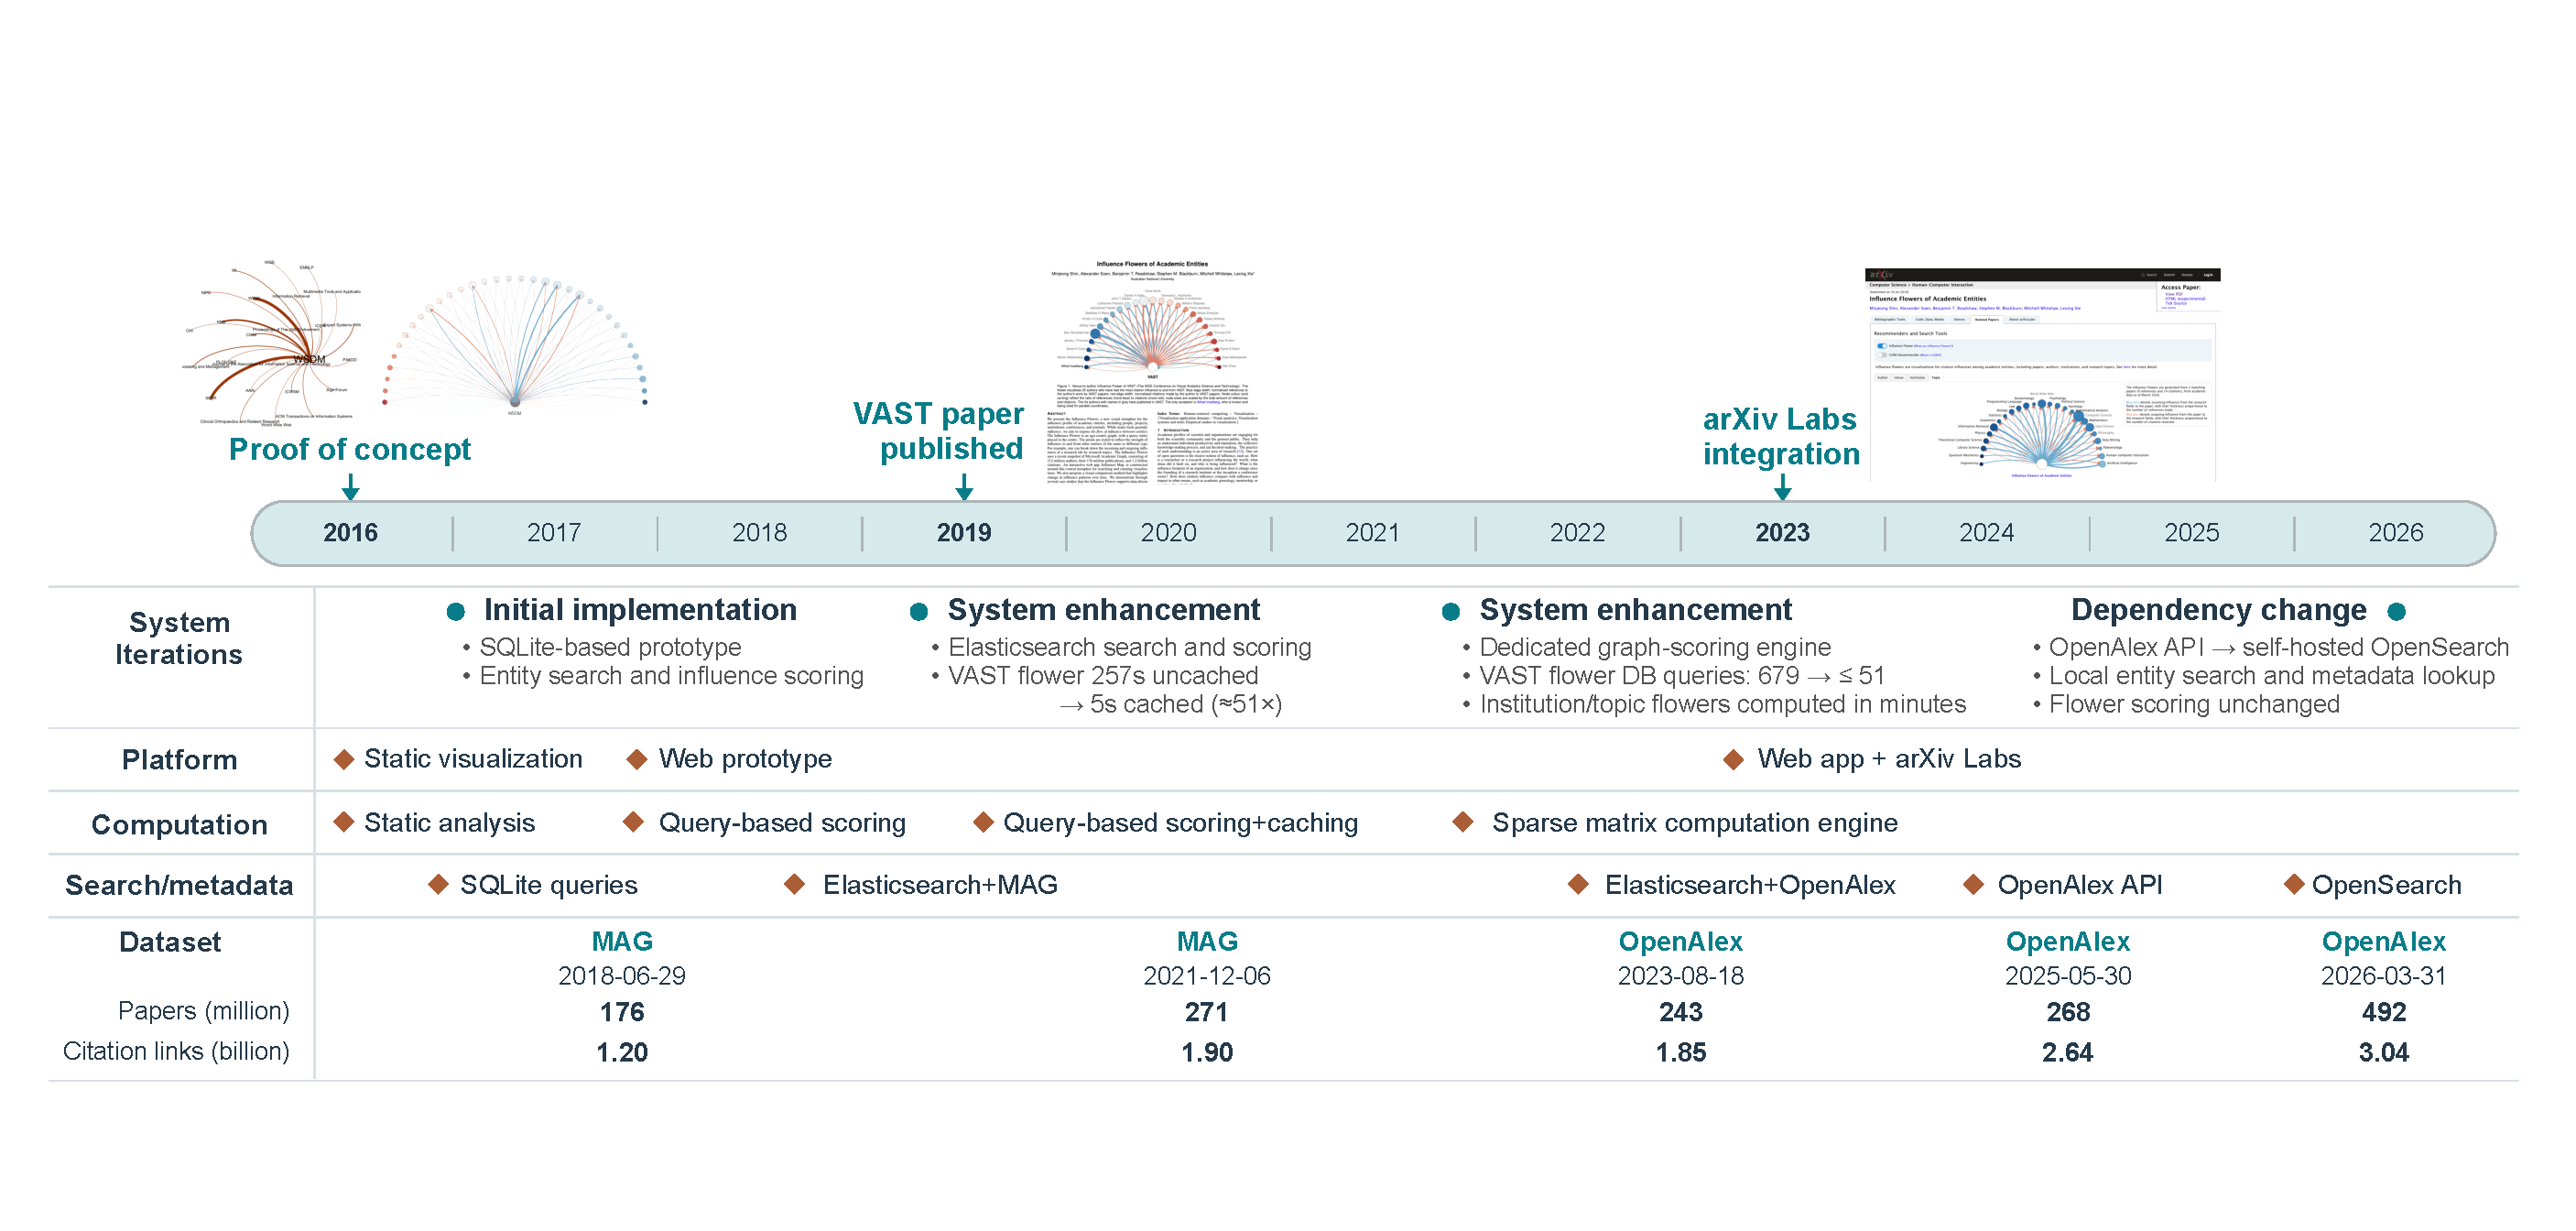
\includegraphics[width=\textwidth]{history.pdf} \\
    \caption{\textbf{Evolution of Influence Flower (2016--2026).} Research and deployment milestones include the initial proof of concept, the VAST publication, and arXiv Labs integration. The rows below the timeline track changes in the platform, computation engine, search and metadata services, and scholarly datasets. Dataset snapshots document the transition from Microsoft Academic Graph (MAG) to OpenAlex, with sizes reflecting the coverage of individual releases. Response times and database-query counts describe distinct performance improvements. The 2026 OpenSearch transition changes search and metadata access while retaining the matrix computation engine.}
    \label{fig:history}
\end{figure}

\textbf{Five Iterations of Influence Flower.}
To address the second question, we will trace the system evolution summarized in \cref{fig:history}, focusing on how successive implementations preserved the flower's analytical purpose under changing technical and operating conditions. The project began with static visual experiments in 2016, followed by a software prototype in 2017. We will organize this history around five iterations: prototyping with SQLite and Microsoft Academic Graph (MAG) (\cite{sinha2015overview}); search and scoring with Elasticsearch; the introduction of a sparse matrix computation engine in 2021; migration to OpenAlex snapshots (\cite{priem2022openalex}) and OpenAlex API for entity search; and the move to self-hosted OpenSearch for entity search and metadata lookup in 2026. For each iteration, we will examine what prompted the change, which adaptation followed, and which components could remain in place.


Quantitative milestones will make this history concrete. In early 2016, we processed approximately 121 million publications and 0.95 billion citation links; by March 2026, the graph contained 492 million works and 3.04 billion citation edges. Intermediate MAG and OpenAlex snapshot sizes appear in \cref{fig:history}, with differences in coverage and entity resolution made explicit.\footnote{Early processing logs and code: \url{https://github.com/lexingxie/academic-graph}; current pipeline: \url{https://github.com/csmetrics/influencemap/}}
% Quantitative milestones will make this history concrete. Our dataset grew from 176 million publications and 1.2 billion citation links in the 2018 MAG snapshot (\cite{shin2019influence}) to 271 million publications and 1.9 billion links in December 2021. Following our transition to OpenAlex, the dataset contained 243 million works and 1.85 billion citation links in August 2023, increasing to 268 million works and 2.64 billion links in May 2025. By March 2026, the citation graph contained 3.04 billion edges. These counts reflect the coverage and entity resolution of each data source.\footnote{Source code and data processing pipeline: \url{https://github.com/csmetrics/influencemap/}}

Performance improvements will illustrate how we adapted the system to this increasing scale. In the Elasticsearch implementation, caching reduced generation time for the VAST flower from 257 seconds on the first request to 5 seconds on reuse (\cite{shin2019influence}).
The sparse matrix computation engine later reducing the VAST query requirement from 679 to 51, primarily for resolving names. For larger entities, the earlier implementation still took over 30 minutes to compute an institution flower even with complete cache entries; the matrix engine made institution and topic flowers feasible within a few minutes, using approximately 30 GB of memory. We will distinguish cache-state timings from query-count reductions and broader scalability observations when discussing these improvements.

The 2023 arXiv Labs integration turned a research artifact into a service embedded in researchers' everyday browsing, making continued availability and predictable costs practical requirements. External changes added pressure: MAG updates ceased after 31 December 2021, prompting migration to OpenAlex,\footnote{\url{https://www.microsoft.com/en-us/research/articles/microsoft-academic-to-expand-horizons-with-community-driven-approach/}} which introduced usage-based API pricing, including charges for search, in 2026.\footnote{\url{https://blog.openalex.org/openalex-api-new-features-and-usage-based-pricing/}} We will examine how access terms, workload, and operating costs reshaped maintenance priorities.

% The arXiv Labs integration, merged in 2023, marked a shift from a research artifact to a service embedded in researchers' everyday browsing. Continued availability and predictable operating costs became part of the project's responsibilities. We will discuss how use beyond the original research setting changed the priorities for maintenance.

% Changes in external data services introduced additional pressures. Microsoft stopped providing updated MAG data after 31 December 2021, prompting our migration to OpenAlex.\footnote{\url{https://www.microsoft.com/en-us/research/articles/microsoft-academic-to-expand-horizons-with-community-driven-approach/}} In 2026, OpenAlex introduced usage-based API pricing, including charges for search.\footnote{\url{https://blog.openalex.org/openalex-api-new-features-and-usage-based-pricing/}} We will examine how these changes made data availability and recurring API costs part of the system's maintenance problem.


\textbf{Implementation Considerations.}
These transitions will ground our discussion of implementation choices. Separating data ingestion, entity search, and flower computation made components replaceable. A preprocessing adapter converted OpenAlex snapshots, with their different identifiers, record structure, and metadata, into the format expected by the existing matrix pipeline. This let the computation layer remain in place during the data-source migration. In 2026, local OpenSearch replaced API-based entity search and metadata lookup, providing control over runtime dependencies and costs while leaving flower computation unchanged.


The engine uses memory-mapped sparse arrays and Numba-compiled kernels to compute flowers on demand. The local sparse representation trades storage and memory demands for fewer runtime database queries, while memory mapping lets the operating system manage access to the arrays. These examples will motivate a discussion of component boundaries, feature simplification, and the trade-offs of local operation: reduced API dependence balanced against indexing, metadata updates, and service maintenance. We will assess these choices against performance, resource demands, and the capacity of a small academic team.

% The computation engine stores the citation graph in memory-mapped sparse arrays and uses Numba-compiled kernels to compute flowers on demand. These examples will motivate a discussion of component boundaries, feature simplification, and the trade-offs of local operation. Reduced dependence on external APIs brings responsibilities for indexing, updating metadata, and maintaining local services. We will discuss these choices in terms of performance, resource requirements, and the maintenance work they create for a small academic team.

% These implementation choices also raise broader questions about sustainable scholarly software. Research papers are designed to become fixed records, and reproducibility often encourages us to freeze code and data alongside them. Public-facing scholarly infrastructure faces the opposite condition: its data sources evolve, APIs disappear or become costly, software dependencies change, traffic grows, and users continue to expect current results. We will contrast the frozen snapshot with living infrastructure and pose the central question of the article: how can living infrastructure be engineered so that change remains inexpensive? Our working answer is that sustainability is not the ability to avoid change, but the ability to absorb inevitable change at a tolerable technical and organizational cost.

Research papers become fixed records, often accompanied by frozen code and data for reproducibility. A public service must also remain useful as data, dependencies, and usage change. We will examine how to preserve reproducible research artifacts alongside a service that continues to evolve. We will draw two lessons from this shift to living infrastructure: design for change by keeping components separable, and design for affordable maintenance by balancing performance with the work and resources needed to sustain the service. We will conclude with the project's lasting 'fruits': reusable infrastructure, engineering knowledge, a community reached through arXiv Labs, and a relational approach to scholarly influence.

% We will draw two broader lessons from these iterations. First, design for change: keep data ingestion, search, and computation separable so that changing a data source or external service does not require rebuilding the entire system. Second, design for affordable maintenance: balance performance and resource demands with the work needed to operate, update, and sustain the service within a small research team's capacity.

% We will conclude by considering the lasting contributions, or "fruits" of a decade of work: reusable infrastructure and engineering knowledge, a community of users reached through arXiv Labs, and a relational approach to studying scholarly influence. These outcomes will frame our broader argument that sustaining a research tool means preserving its analytical purpose while keeping its implementation affordable to adapt.

% All references should be stored in the file "references.bib"
% Please do not modify anything below this line.
\printbibliography


\end{document}
